\section*{Position and Momentum: Eigenfunctions and Operators\sectionmark{Position and Momentum}}

	Two particularly useful operators in quantum mechanics are the position operator, $\hat x$, and the momentum operator, $\hat p$.
	
	In this set of exercises, we will consider what these operators and their eigenfunctions look like in the position representation.
	
	\vspace{0.25in}
	
	\begin{questions}
		\question An eigenstate of the position operator is one where the probability of finding the particle is nonzero at only one position.
		
			\begin{parts}
				\part Predict what the position eigenfunction for a particle found at $x=x_0$ should look like:
				
\vspace{0.5in}					\centerline{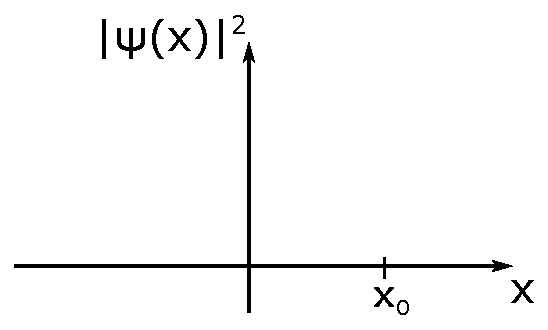
\includegraphics[width=0.5\textwidth]{includes/xp-eigenfuns-eigenvals-FIGURES/x0_axes}}		
\vspace{0.3in}		
				
				\part The eigenvalue of this position eigenstate should be the particle's position, e.g. $x_0$. What operator might you be able to apply to extract the value of $x_0$?
				
					\begin{solution}[3.3in]
					\end{solution}
			
			\end{parts}
			
			
		\begin{flushright}(Continued on back of page $\rightarrow$)	\end{flushright}
		\newpage 
		\item De Broglie told us that a particle with momentum $p$ has wavelength $\lambda = \frac{h}{p}$.
		
			\begin{parts}
				\part One useful function that has a wave-like form is $f(x) = e^{ikx} = \cos(kx) + i\sin(kx)$.  What is the wavelength of this function in terms of $k$ (i.e. for what value of $\lambda$ does $f(x+\lambda) = f(x)$)?
				
					\begin{solution}[2in]
					\end{solution}
				
				\part Set this wavelength equal to de Broglie's value for $\lambda$. How is $k$ related to $p$?
				
					\begin{solution}[2in]
					\end{solution}
				
				
				\part What operator might you be able to apply to the function $e^{ikx}$ to extract the momentum eigenvalue $p$?
				
					\begin{solution}[2in]
					\end{solution}
				
			\end{parts}
	\end{questions}